%%%%%%%% ICML 2018 EXAMPLE LATEX SUBMISSION FILE %%%%%%%%%%%%%%%%%

\documentclass{article}

% Recommended, but optional, packages for figures and better typesetting:
\usepackage{microtype}
\usepackage{graphicx}
\usepackage{subfigure}
\usepackage{booktabs} % for professional tables
\usepackage{amsfonts}
\usepackage{amsmath}

% hyperref makes hyperlinks in the resulting PDF.
% If your build breaks (sometimes temporarily if a hyperlink spans a page)
% please comment out the following usepackage line and replace
% \usepackage{icml2018} with \usepackage[nohyperref]{icml2018} above.
\usepackage{hyperref}

% Attempt to make hyperref and algorithmic work together better:
\newcommand{\theHalgorithm}{\arabic{algorithm}}

% Use the following line for the initial blind version submitted for review:
%\usepackage{icml2018}

% If accepted, instead use the following line for the camera-ready submission:
\usepackage[accepted]{icml2018}

% The \icmltitle you define below is probably too long as a header.
% Therefore, a short form for the running title is supplied here:
\icmltitlerunning{Warfarin Dosage Prediction with LinUCB and Logistic Regression}

\begin{document}

\twocolumn[
\icmltitle{Warfarin Dosage Prediction with LinUCB and Logistic Regression}

% It is OKAY to include author information, even for blind
% submissions: the style file will automatically remove it for you
% unless you've provided the [accepted] option to the icml2018
% package.

% List of affiliations: The first argument should be a (short)
% identifier you will use later to specify author affiliations
% Academic affiliations should list Department, University, City, Region, Country
% Industry affiliations should list Company, City, Region, Country

% You can specify symbols, otherwise they are numbered in order.
% Ideally, you should not use this facility. Affiliations will be numbered
% in order of appearance and this is the preferred way.
\icmlsetsymbol{equal}{*}

\begin{icmlauthorlist}
\icmlauthor{Haojun Li}{stanford}
\end{icmlauthorlist}

\icmlaffiliation{stanford}{Department of Computer Science, Stanford University, CA, USA}
\icmlcorrespondingauthor{Haojun Li}{haojun@stanford.edu}
% You may provide any keywords that you
% find helpful for describing your paper; these are used to populate
% the "keywords" metadata in the PDF but will not be shown in the document
\icmlkeywords{Machine Learning, ICML}

\vskip 0.3in
]

% this must go after the closing bracket ] following \twocolumn[ ...

% This command actually creates the footnote in the first column
% listing the affiliations and the copyright notice.
% The command takes one argument, which is text to display at the start of the footnote.
% The \icmlEqualContribution command is standard text for equal contribution.
% Remove it (just {}) if you do not need this facility.

\printAffiliationsAndNotice{}  % leave blank if no need to mention equal contribution
%\printAffiliationsAndNotice{\icmlEqualContribution} % otherwise use the standard text.

\begin{abstract}
	Predicting the correct dosage of Warfarin usually requires many trial-and-errors, and correct dosage found for one patient cannot be immediately used to predict the correct dosage for the next patient using traditional methods. However, due to Reinforcement Learning's fast ability to learn and adapt to new data, we can make more accurate decisions as we see more and more patients and incorporate them immediately in predicting the dosage for the next patient. In this report I model this problem as a Stochastic Linear Bandit problem and uses Disjoint LinUCB algorithm to predict the dosage range given patient features. This method outperforms 2 baselines (Fixed Dosage and Clinical Dosing Algorithm) in terms of regret. I also provide a supervised version of the algorithm, and shows that it outperforms all other methods in terms of regret, but not fraction of incorrect dosages against Clinical Dosing Algorithm due to problem construction. 
\end{abstract}

\section{Introduction}
Warfarin is a blood thinner commonly used to treat a variety of blood clots. Since it is difficult to accurately prescribe the appropriate dose of Warfarin to patients, many researchers have attempted this problem with a variety of algorithms and data. \cite{international2009estimation} However, most of these approaches are based on a supervised dataset obtained from existing patients with known correct dosage of Warfarin. These gold labels of correct Warfarin dosage is obtained through trial and error (give a low dosage in the beginning and gradually increase the dosage until we find the correct one). These methods perform very well in practice, but a main drawback of these algorithms is that it requires an initial period of trial and error. This means that the next patient who needs to be treated with Warfarin cannot benefit from the information learned from the patient immediately before it. Reinforcement Learning, on the other hand, allows us to constantly update our estimation based on observations of the previous predicted dose. Thus, it is an attractive algorithm in finding the correct dosage of Warfarin in an ongoing medial trial.

Reinforcement Learning has applications in many fields ranging from robotics \cite{peters2003reinforcement} to advertisement bidding \cite{cai2017real}. Its ability to learn information in real-time is particularly attractive to problems where an agent can interact with an environment and gather real time data. It has allowed researchers to move beyond rule-based systems and instead use a data-driven approach to improve systems in real time. Another advantage of these algorithms is that it is sometimes able to achieve super human performance, especially in video games \cite{mnih2013playing}. However, many challenges remain for these algorithms. For example, most of them require substantial amount of trial and error in order for the agent to learn an optimal policy. In \citet{mnih2013playing} for example, the agent has to play millions of games before achieving reasonable performance, and eventually achieving super human performance. An attempt to address this problem is using imitation learning \cite{codevilla2018end} to learn a policy by mimicking human behavior. Another approach is to bound the regret theoretically, such as the UCB algorithm \cite{lai1985asymptotically}, which balances exploration and exploitation, achieving better results in situations where trying millions of times is not an option. These so called "multi-arm bandit" problem formulation is widely used in online advertising due to its ability to (eventually) behaving optimally while exploring a reasonable amount of time. A specific type of bandit problem called "stochastic linear bandits" \cite{abe2003reinforcement} allows us to also incorporate context in decision making, making bandit problems more realistic in problems where observations and actions can be featurized and incorporated into the agent's decision making process. 

\section{Related Works}
There are many algorithms introduced over the years in providing better bounds for the regret for stochastic linear bandit problems. The classic algorithms such as one introduced in \citet{auer2002using} as well as later works to improve upon the upper bound in \citet{dani2008stochastic} both attempted to find a good algorithm that gives polylog(T) regret. Other works adapted the algorithms to other practical domains, such as \citet{li2010contextual}, which introduces the LinUCB algorithm that we will be experimenting with in this report. Other methods that were adapted to classic multi-arm bandits such as Thompson Sampling have been adapted to contextual bandits with linear payoffs as well \cite{agrawal2013thompson}. For more information related to more algorithms in linear bandits, please refer to the book \citet{lattimore2018bandit} as well as the default project handout.

\section{Approach}
\subsection{Problem Definition}
The problem definition is the same as the default project handout. Please refer to the handout for more information.

\subsection{Baselines}
\label{baseline}
The baselines are as defined in the default project handout. We will chose the first 2 baselines to compare, namely a \textit{Fixed dose} baseline as well as a \textit{Warfarin Clinical Dosing Algorithm} baseline. The former is a baseline that prescribes medium dose (21-49 mg/week) while the latter is an algorithm that predicts the dosage based on some features of the patient. To make comparison fair to the baseline, all feature-based algorithm introduced below as well as regret calculations will be using the same set of feature classes: \textbf{Race, Age in decades, Height (cm), Weight (kg), Carbamazepine (Tegretol), Amiodarone (Cordarone), Phenytoin (Dilantin), Rifampin or Rifampicin}.

\subsection{LinUCB}
The LinUCB algorithm that we will adapt is introduced in \citet{li2010contextual}. We will adapt the "LinUCB with disjoint linear models". We did not experiment with Hybrid models since there is no additional context shared among different arms, but rather the decision to pull each arm can be seen as independent. According to the original paper, the benefit of the hybrid model is that it will understand context similarities between arms, which does not apply to our problem.
\begin{algorithm}[tbh]
	\caption{Adapted Disjoint LinUCB}
	\label{alg:linucb}
	\begin{algorithmic}
		\STATE {\bfseries Input:} $\alpha\in\mathbb{R}^+$
		\STATE Initialize $\mathbf{A}_a\leftarrow\mathbf{I}_d$ for all $a\in$ \{low, medium, high\}
		\STATE Initialize $\mathbf{b}_a\leftarrow\mathbf{0}_{d\times 1}$ for all $a\in$ \{low, medium, high\}
		\FOR{$T=1, 2, 3, \cdots, T$}
		\FOR{$a\in$\{low, medium, high\}}
		\STATE $\hat{\beta}_a \leftarrow \mathbf{A}_a^{-1}\mathbf{b}_a$
		\STATE $p_{t, a}\leftarrow \hat{\beta}_a^\top \mathbf{x}_{t, a} + \alpha\sqrt{\mathbf{x}_{t, a}^\top\mathbf{A}_a^{-1}\mathbf{x}_{t, a}}$
		\ENDFOR
		\STATE $a_t = \arg\max_{a\in\{low, medium, high\}} p_{t, a}$ and observe $r_t$
		\STATE $\mathbf{A}_{a_t}\leftarrow \mathbf{A}_{a_t} + \mathbf{x}_{t, a_t}\mathbf{x}_{t, a_t}^T$
		\STATE $\mathbf{b}_{a_t}\leftarrow \mathbf{b}_{a_t} + r_t \mathbf{x}_{t, a_t}$
		\ENDFOR
	\end{algorithmic}
\end{algorithm}

Since we know that there are only 3 arms to pull, we can initialize the matrix beforehand. The rest of the algorithm is exactly the same as in the original paper. However, the original author of the paper provided $\alpha = 1 + \sqrt{\ln(2/\delta)/2}$ as the input of the algorithm given $\delta$. However, further investigation below shows that different $\alpha$'s yield different results given our horizon. In particular, smaller $\alpha$ leads to earlier exploitation, which yields a worse regret bound in exchange for minimizing short term regret. This is particularly useful given our problem since we have a short horizon (only 5528 patients). This also leads us to adopt smaller set of features since we hypothesize that a higher set of features will lead the agent to explore more due to its optimistic nature.

\subsection{Supervised Learning}
\label{supervised_learning_approach}
We also adopt a supervised learning approach. Since we have the correct dosage category for each patient, it seems like a waste to not be able to use it. We will use Softmax Regression to fit the features defined in section \ref{baseline} in bold with a batch size of 50. In essence, for every 50 patients we will add them to our memory and refit the model on all the patients we have seen so far. The generic algorithm that works with any supervised model class is described in detail below
\begin{algorithm}[tbh]
	\caption{Supervised Learning}
	\label{alg:linucb}
	\begin{algorithmic}
		\STATE {\bfseries Input:} Batch Size $b$
		\STATE Initialize A list of patient features $X_0$ and labels $y_0$
		\FOR{$t=1, 2, 3, \cdots, T$}
		\IF{$T < b$}
		\STATE $X_t \leftarrow X_{t-1} + [x_{t}]$
		\STATE select $a_t = $ medium, observe $r_t$ and label $y_t$
		\STATE $y_T \leftarrow y_{t-1} + [y_t]$
		\ENDIF
		\IF{$t \bmod b == 0$}
		\STATE Fit supervised predictor $f_{\lfloor t/b\rfloor}$ to $X_{t-1}$ and $y_{t-1}$
		\ENDIF
		\STATE select $a_t = f_{\lfloor t/b\rfloor}(x_t)$, observe $r_t$ and label $y_t$
		\STATE $X \leftarrow X + [x_{t}]$
		\STATE $y \leftarrow y + [y_t]$
		\ENDFOR
	\end{algorithmic}
\end{algorithm}

The batch size can be tuned depending on how frequently we want to update. Faster updates means that we can adapt quicker to new data, but also means that we might have more noisy predictions due to this fast adaptation.

\subsection{Regret}

To calculate regret, we first fit a linear model on the features selected in section \ref{baseline} in bold text as well as the actual reward (-1 for a failed prediction and 0 otherwise) for each action (low, medium, high). Then, we use the coefficients derived from the linear model to get the predicted reward for each dosage category for each patient in our dataset $\beta_a^\top x_i$. To calculate empirical regret, we simply sum the regret for each predicted action against the action with the highest $\beta_a^\top x_i$. Specifically, the total regret for a sequence of actions $\mathbf{a}$ on the patient features $X$ is 
\begin{equation}
	\text{regret}_{X, \mathbf{a}} = \sum_{t=1}^T \max_{a'\in\{low, medium, high\}}\beta_{a'}^\top x_t - \beta_{a_t}^\top x_t
\end{equation}

\section{Experiment Results}
\subsection{LinUCB}
\subsubsection{Alpha Search}
\label{alpha_search}
Finding the correct exploration bonus term is important since we have a shorter horizon. Thus, it may be better to commit early to a policy that we believe will do sufficiently well rather than keep exploring hoping for a better policy. Thus, a lower exploration bonus means lower average total regret but could lead to sub-optimal solutions. Here we compare the 2 metrics (average fraction of incorrect dosages and average total regret) of each $\alpha$ value. 
\begin{figure}
	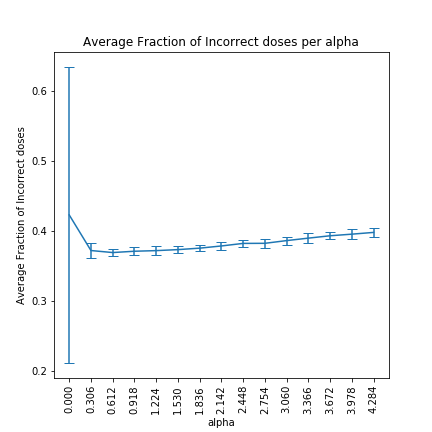
\includegraphics[width=\linewidth]{../plots/avg_frac_incorrect_alpha.png}
	\caption{Average fraction of incorrect doses for each $\alpha$ value. There are 20 trials run for each alpha value. Fraction of incorrect cases are plotted with 95\% confidence interval}
	\label{fig:avg_frac_incorrect_alpha}
\end{figure}

\begin{figure}
	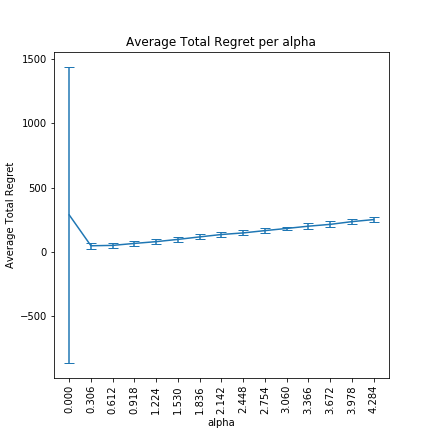
\includegraphics[width=\linewidth]{../plots/avg_tot_regret_alpha.png}
	\caption{Average total regret for each $\alpha$ value. There are 20 trials run for each alpha value. Averages of total regret are plotted with 95\% confidence interval}
	\label{fig:avg_tot_regret_alpha}
\end{figure}

\begin{figure}
	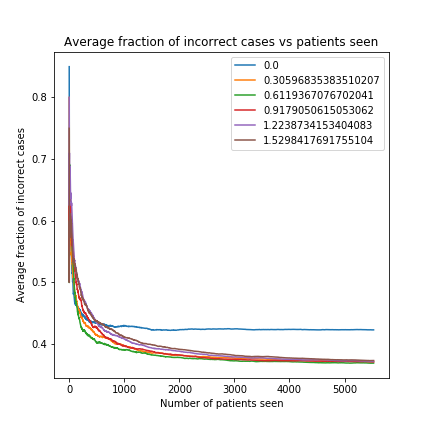
\includegraphics[width=\linewidth]{../plots/avg_frac_alphas.png}
	\caption{Average fraction incorrect cases as the algorithm sees more patients. Each $\alpha$ value simulation is run 20 times and the fraction of incorrect dosages is averaged across these 20 runs at each "time stamp". 95\% confidence interval not displayed to minimize clutter}
	\label{fig:avg_frac_alphas}
\end{figure}

If the $\alpha$ value is 0.0, which means that we have no exploration bonus, then we are basically running a greedy strategy. We estimate the value for each patient and immediately apply that information to the next patient. Thus, we have a huge variation of fraction of incorrect cases and average total regret as seen in figure \ref{fig:avg_frac_incorrect_alpha} and \ref{fig:avg_tot_regret_alpha}. The confidence interval of the average of the 2 metrics across 20 trials is very large. In addition to that, as seen in figure \ref{fig:avg_frac_alphas}, we committed to a policy too early and was unable to find the optimal solution later on, achieving much worse average fraction of incorrect doses as the algorithm sees more patients.

Another important result is that lower $\alpha$ does usually means better average total regret but also means that we could have committed to a policy too early (which explains the lower average fraction of incorrect doses). As seen in figure \ref{fig:avg_frac_alphas}, a lower $\alpha$ not only lead to sub-optimal decisions (like $\alpha=0.0$) but even when we eventually achieve optimal parameters, it committed to a strategy too early and thus it takes more time to rectify that mistake since we are exploring so little. Thus, finding the correct $\alpha$ is a balance between the 2. The best alpha found is $0.612$ which achieved an average total regret of $51.45$ and fraction of incorrect cases at $0.3692$. These results comparing to the baseline results will be shown later.


\subsubsection{Robustness}
In order to verify that the model is robust to the permutation of patients, we have run all LinUCB experiments for 20 trials with different permutations of patients. As we can see in figure \ref{fig:avg_regret_per_t} and \ref{fig:frac_incorrect_dosage_t}, we achieved fairly stable average regret per patient of around 0.009 (average total regret of 51.45) and fraction of incorrect dosages around 0.37. This not only mean that our results are statistically sound, it also means that our model is very robust across different permutation of patients judging by the stable results.

\begin{figure}
	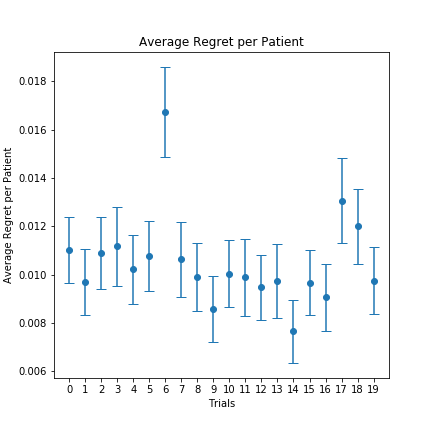
\includegraphics[width=\linewidth]{../plots/avg_regret_per_t.png}
	\caption{Expected regret per patient across 20 trials for $\alpha=0.612$. Plotted with 95\% confidence interval with t-statistic}
	\label{fig:avg_regret_per_t}
\end{figure}

\begin{figure}
	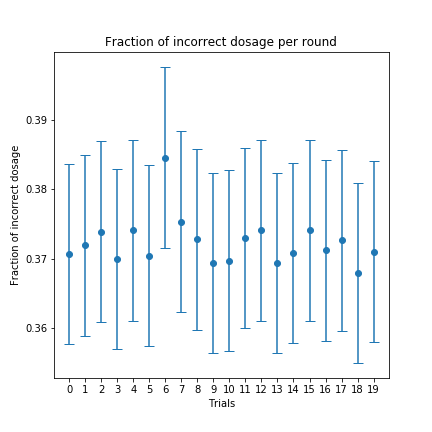
\includegraphics[width=\linewidth]{../plots/frac_incorrect_dosage_t.png}
	\caption{Expected value of incorrectness of dosage across 20 trials $\alpha=0.612$. Plotted with 95\% confidence interval with t-statistic}
	\label{fig:frac_incorrect_dosage_t}
\end{figure}

\subsection{Supervised Methods}

\subsubsection{Upper limit of performance}
\label{supervised_upper_limit}
For supervised methods, we used 2 different kind of supervised learning model classes, namely SVM and Multinomial Logistic Regression (aka Softmax Regression). Since the algorithm can receive the correct Warfarin dosage as part of its training and not just rewards of correct/incorrect dosages, these algorithms should in theory do much better than the RL-based methods. Indeed, they do very well comparing to the results shown above.  However, we are first interested in seeing the potential optimal of different model classes in order to chose the best one. These upper limits are derived by fitting the model on the entire dataset with correct labels, and evaluating them on the same dataset and observe the regret and fraction of incorrect Warfarin doses. In tabel \ref{table:supervised_optim} we can clearly see that logistic regression does so much better in terms of both optimal regret as well as optimal fraction of incorrect warfarin doses. We suspect the reason being that logistic regression is a more powerful model in this specific case because the correct dosage does seem to have a linear relationship with the features.

\subsubsection{Supervised Results}
\label{supervised_results}
We have also run this model several times and we found that with a batch size of 50, the supervised model described in section \ref{supervised_learning_approach} achieve a total regret of $33.49$ and a fraction of incorrect cases $0.3598$. Interestingly this does beat the clinical algorithm in terms of regret, but it does not beat the clinical algorithms in terms of total incorrect cases. In terms of regret, since the supervised model is linear, it is able to find better parameters for each dosage category than a linear regression predictor such as the Clinical Dosing Algorithm. However, as shown in section \ref{supervised_upper_limit} and table \ref{table:supervised_optim}, it is not a limitation of the model but rather a limitation of the batched method. The agent can only see 50 patients at a time, and only after certain amount of patients does it have a good estimate for each of the parameters.

\begin{table}[t]
	\caption{Table of Model Class and their optimal regret and Opitmal fraction of incorrect doses. Obtained by training the model on the entire dataset and evaluating it on the entire dataset}
	\label{table:supervised_optim}
	\vskip 0.15in
	\begin{center}
		\begin{small}
			\begin{sc}
				\begin{tabular}{lccc}
					\toprule
					Model Class         & Optimal Regret & Optimal Fraction\\
					\midrule
					Logistic & \textbf{30.93}          & \textbf{0.3538}  \\
					SVM                 & 61.53          & 0.3882 \\
					\bottomrule
				\end{tabular}
			\end{sc}
		\end{small}
	\end{center}
	\vskip -0.1in
\end{table}

\subsection{Comparison Across All Methods}
Here we compare results across all methods. They are summarized in table \ref{table:comparison}. As we can see from the table, all the new methods tried are able to beat the Fixed Dose baseline method in terms of average total regret and average fraction of incorrect doses. The supervised logistic regression method with a batch size of 50 achieved the least regret. However, it is still not able to beat the Clinical Dosing algorithm in terms of average fraction of incorrect dosages. Still, as shown in section \ref{supervised_results}, this is not a limit of the model class but rather a limit to the problem setting where patients come one at a time while Clinical Dosing algorithm does not have this "exploration period". The LinUCB Disjoint model is able to beat both baselines in terms of average total regret, but it was not able to achieve better fractions of incorrect dosages due to its exploration period.
\\

\begin{table}[t]
	\caption{Table of comparison across methods}
	\label{table:comparison}
	\vskip 0.15in
	\begin{center}
		\begin{small}
			\begin{sc}
				\begin{tabular}{lccc}
					\toprule
					Method          & Avg Total Regret & Avg Fraction    \\
					\midrule
					Fixed Dose      & 61.53            & 0.3882          \\
					Clinical Dosing & 54.227           & \textbf{0.3572} \\
					LinUCB          & 51.45            & 0.3692          \\
					Logistic        & \textbf{33.49}   & 0.3598    	\\
					\bottomrule
				\end{tabular}
			\end{sc}
		\end{small}
	\end{center}
	\vskip -0.1in
\end{table}


\subsubsection{Performance Analysis}
\begin{figure}
	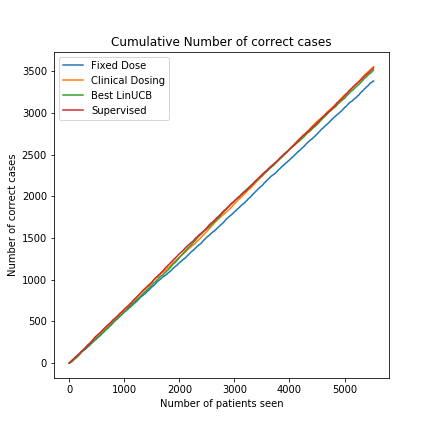
\includegraphics[width=\linewidth]{../plots/comparison.png}
	\caption{A comparison of algorithms and their trajectory in terms of number of correct dosage predictions. We picked the best performing run of each algorithm in composing this figure}
	\label{fig:comparison}
\end{figure}

\begin{figure}
	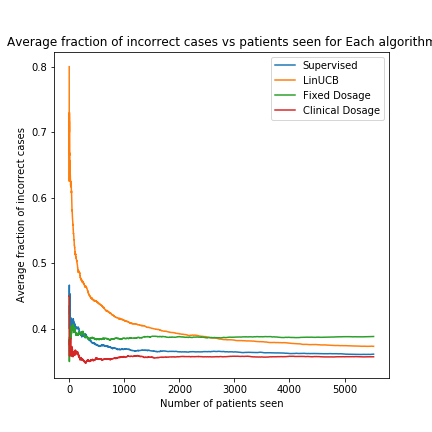
\includegraphics[width=\linewidth]{../plots/avg_frac_algos.png}
	\caption{A comparison of algorithms and the fraction of correct cases as they start seeing more patients. Each algorithm is run 20 times and the fraction of incorrect dosages is averaged across these 20 runs at each "time stamp". 95\% confidence interval not displayed to minimize clutter}
	\label{fig:comparison_frac}
\end{figure}

A better way of understanding the performance of these algorithms is to see the types of decisions they make for each patient as it learns more about the patients. Plotted in figure \ref{fig:comparison} is a comparison of algorithms in terms of cumulative number of correct decisions made by the algorithm as it sees more patients and gain a better understanding of the patients. These are plotted by selecting the run with the highest rewards in order to compare their maximum performances. As we can see from the plot, the fixed dose method performed very poorly and the number of correct cases grows linearly with time. The Supervised learning method with Logistic regression had the most consistent trajectory across all algorithms. As you can see from the Green line (the best run of a LinUCB algorithm), it spends some time initially performing below the Clinical Dosing and Supervised algorithms because it is exploring rewards for different dosages. Notably, it performs worse than fixed dosages in the beginning. Then, after finding good parameters, it quickly caught up to other algorithms and sometimes surpassing them. This is what we expected to see in this graph.

Another way of showing this is to display the average fraction of incorrect cases as we see more patients across 20 different permutation of patients much like those in section \ref{alpha_search}. As we can see from figure \ref{fig:comparison_frac}, clinical dosage start correctly predicting cases almost immediately due to the fact that it is a fixed policy with good parameters. Fixed Dosage also perform very well in the beginning because they have no exploration period. This also means that their performance is fixed throughout the entire run. On the other hand, LinUCB algorithm had an initial period of exploration (which is why it is doing poorly) and eventually the fraction of incorrect cases drops after it has a good estimate of the parameters. However, the initial period of exploration means that we will have a lot of failed cases in the beginning, and that inflates the number of total incorrect cases. The supervised learning approach also did fairly well. After an initial period of uncertainty, it quickly converged to very good parameters, but still fell short in beating the Clinical Dosage baseline. 

\section{Conclusion}

Both the LinUCB method and the supervised methods performed well comparing to very strong baselines. Both methods beat both baselines in terms of average total regret, but both fell short in beating the clinical dosing algorithm in terms of average fraction of incorrect cases. Due to the fact that these algorithms require a short exploration period before being able to converge to good parameters, while clinical dosage algorithms is able to make correct predictions right away. Still it did do sufficiently well in approximating the clinical dosage baseline. Analysis showed that for short horizon problems like these, it is better to chose a smaller $\alpha$ value so that we commit to a strategy early instead of exploring more in order to find a better policy.

\section{Team Contributions}
I myself completed this project by myself with extra support from Haojun Li (myself) 

% In the unusual situation where you want a paper to appear in the
% references without citing it in the main text, use \nocite

\bibliography{paper}
\bibliographystyle{icml2018}

\end{document}


% This document was modified from the file originally made available by
% Pat Langley and Andrea Danyluk for ICML-2K. This version was created
% by Iain Murray in 2018. It was modified from a version from Dan Roy in
% 2017, which was based on a version from Lise Getoor and Tobias
% Scheffer, which was slightly modified from the 2010 version by
% Thorsten Joachims & Johannes Fuernkranz, slightly modified from the
% 2009 version by Kiri Wagstaff and Sam Roweis's 2008 version, which is
% slightly modified from Prasad Tadepalli's 2007 version which is a
% lightly changed version of the previous year's version by Andrew
% Moore, which was in turn edited from those of Kristian Kersting and
% Codrina Lauth. Alex Smola contributed to the algorithmic style files.
